\documentclass[12pt, twoside]{article}
\usepackage[letterpaper, margin=1in, headsep=0.5in]{geometry}
\usepackage[english]{babel}
\usepackage[utf8]{inputenc}
\usepackage{amsmath}
\usepackage{amsfonts}
\usepackage{amssymb}
\usepackage{tikz}
\usetikzlibrary{quotes, angles}
\usepackage{graphicx}
\usepackage{enumitem}
\usepackage{multicol}

\newif\ifmeta
\metatrue %print standards and topics tags

\title{Regents Geometry}
\author{Chris Huson}
\date{September 2020}

\usepackage{fancyhdr}
\pagestyle{fancy}
\fancyhf{}
\renewcommand{\headrulewidth}{0pt} % disable the underline of the header
\raggedbottom


\fancyhead[LE]{\thepage}
\fancyhead[RO]{\thepage \\ Name: \hspace{4cm} \,\\}
\fancyhead[LO]{BECA / Dr. Huson / Geometry 07-Similarity\\* pset ID: 118}

\begin{document}

\subsubsection*{7-8DN-Exam-followup}
\begin{enumerate}
\item Given isosceles $\triangle ABC$ with $\overline{AB} \cong \overline{BC}$, $m\angle B = 53$. Mark and label the diagram, and then find $m\angle A$. \hfill (\emph{the diagram is not to scale})
    \begin{flushright}
    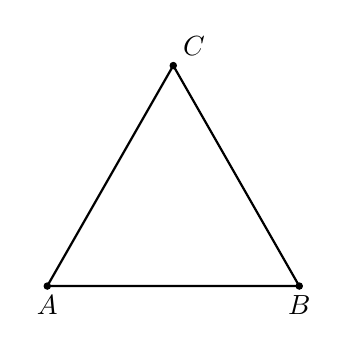
\begin{tikzpicture}[scale=0.8]
      \draw [thick](0,0)--(4,0)--(2,3.5)--(0,0);
      \draw [fill] (0,0) circle [radius=0.05] node[below]{$A$};
      \draw [fill] (4,0) circle [radius=0.05] node[below]{$B$};
      \draw [fill] (2,3.5) circle [radius=0.05] node[above right]{$C$};
    \end{tikzpicture}
    \end{flushright}

\item A series of transformations maps $\triangle ABC$ onto $\triangle DEF$. Circle True or False.
    \begin{enumerate}[itemsep=1cm]
      \begin{multicols}{2}
        \item T \quad F \quad Only rigid motions were applied.
        \item T \quad F \quad $\overline{BC} \rightarrow \overline{EF}$
        \item T \quad F \quad The orientation of the two triangles are reversed.
        \item T \quad F \quad $\overline{AB} \cong \overline{EF}$  \begin{flushright}
        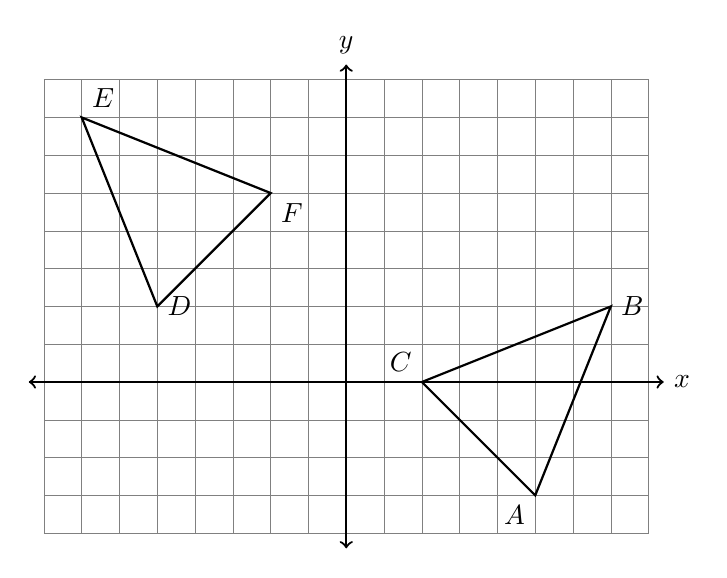
\begin{tikzpicture}[scale=.48]
          \draw [help lines] (-8,-4) grid (8,8);
          \draw [thick, <->] (-8.4,0) -- (8.4,0) node [right] {$x$};
          \draw [thick, <->] (0,-4.4)--(0,8.4) node [above] {$y$};
          \draw [thick]
            (5,-3) node[below left] {$A$}--
            (7,2) node[right] {$B$}--
            (2,0) node[above left] {$C$}--cycle;
          \draw [thick]
            (-5,2) node[right] {$D$}--
            (-7,7) node[above right] {$E$}--
            (-2,5) node[below right] {$F$}--cycle;
        \end{tikzpicture}
        \end{flushright}
      \end{multicols}
    \end{enumerate} 
    
\item The line $\overleftrightarrow{AB}$ has the equation $y=-\frac{2}{3}x+4$. Apply a dilation mapping $\overleftrightarrow{AB} \rightarrow \overleftrightarrow{A'B'}$ with a factor of $k=1.5$ centered at the origin. Draw and label the image on the grid. Write the equation of the line $\overleftrightarrow{A'B'}$.
    \begin{flushright} %4 quadrant regents grid w T-Chart
    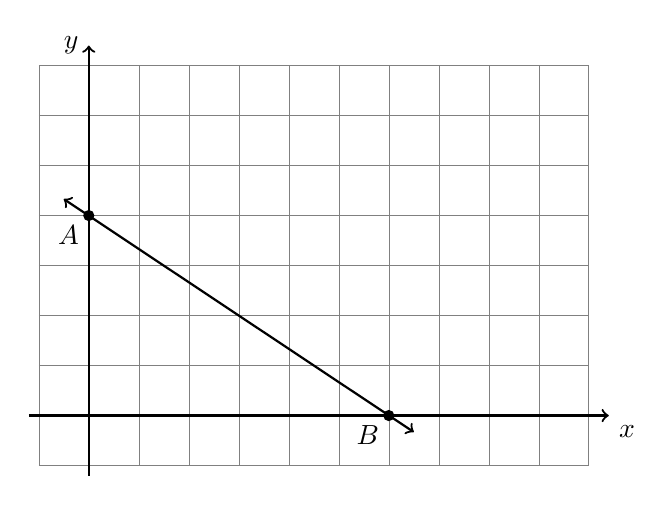
\begin{tikzpicture}[scale=.635]
      \draw [help lines] (-1,-1) grid (10,7);
      \draw [thick, ->] (-1.2,0) -- (10.4,0) node [below right] {$x$};
      \draw [thick, ->] (0,-1.2)--(0,7.4) node [left] {$y$};
      \draw [<->, thick] (-0.5,4.33)--(6.5,-0.33);
      \draw [fill] (0,4) circle [radius=0.1]node[below left]{$A$};
      \draw [fill] (6,0) circle [radius=0.1]node[below left]{$B$};
    \end{tikzpicture}
    \end{flushright}

\newpage
\item The slopes of two lines are given with statements about whether they are parallel or perpendicular. Circle True or False for each statement. Then chose one correct statement and copy it in the space provided.
  \begin{multicols}{2}
    $\displaystyle m_1=2$ \\
    $\displaystyle m_2=\frac{1}{2}$
  \end{multicols}
    \begin{enumerate}[leftmargin=!,labelindent=-0.5cm,itemindent=-2.9cm,itemsep=0.25cm]
      \item True \quad False \quad Parallel. The slopes are equal.
      \item True \quad False \quad Perpendicular. The slopes are  negative reciprocals.
      \item True \quad False \quad Neither. The slopes are not equal and they are not negative reciprocals.
      \item True \quad False \quad Parallel. $\displaystyle 2= \frac{1}{2}$
      \item True \quad False \quad Perpendicular. $\displaystyle 2 \times \frac{1}{2}= -1$
      \item True \quad False \quad Neither. $\displaystyle 2 \neq \frac{1}{2}$ and $\displaystyle 2 \times \frac{1}{2} \neq -1$
    \end{enumerate}
    Copy one correct statement here: \vspace{2cm}
\item Circle True or False for each statement.
  \begin{multicols}{2}
    $\displaystyle m_1=\frac{2}{3}$ \\
    $\displaystyle m_2=-\frac{3}{2}$
  \end{multicols}
    \begin{enumerate}[leftmargin=!,labelindent=-0.5cm,itemindent=-2.9cm,itemsep=0.25cm]
      \item True \quad False \quad Parallel. The slopes are equal.
      \item True \quad False \quad Perpendicular. The slopes are  negative reciprocals.
      \item True \quad False \quad Neither. The slopes are not equal and they are not negative reciprocals.
      \item True \quad False \quad Parallel. $\displaystyle \frac{2}{3}=-\frac{3}{2}$
      \item True \quad False \quad Perpendicular. $\displaystyle \frac{2}{3} \times -\frac{3}{2}= -1$
      \item True \quad False \quad Neither. $\displaystyle \frac{2}{3} \neq -\frac{3}{2}$ and $\displaystyle \frac{2}{3} \times -\frac{3}{2} \neq -1$
    \end{enumerate}
    Copy one correct statement here:

\newpage
\item Shown below is line $l_1$ through the points $A(0,6)$ and $B(0,3)$.
    \begin{enumerate}[itemsep=2cm]
      \begin{multicols}{2}
          \item Find the slope of the line $l_1$.
          \item Write down the equation of the line.
          \item A second line $l_2$ is perpendicular to $l_1$ and passes through $C(2,2)$.\\[0.3cm] 
          Mark and label point $C$ and draw the line $l_2$. 
          \item Write down the equation of the line $l_2$. \vspace{3cm}
        \begin{center}
          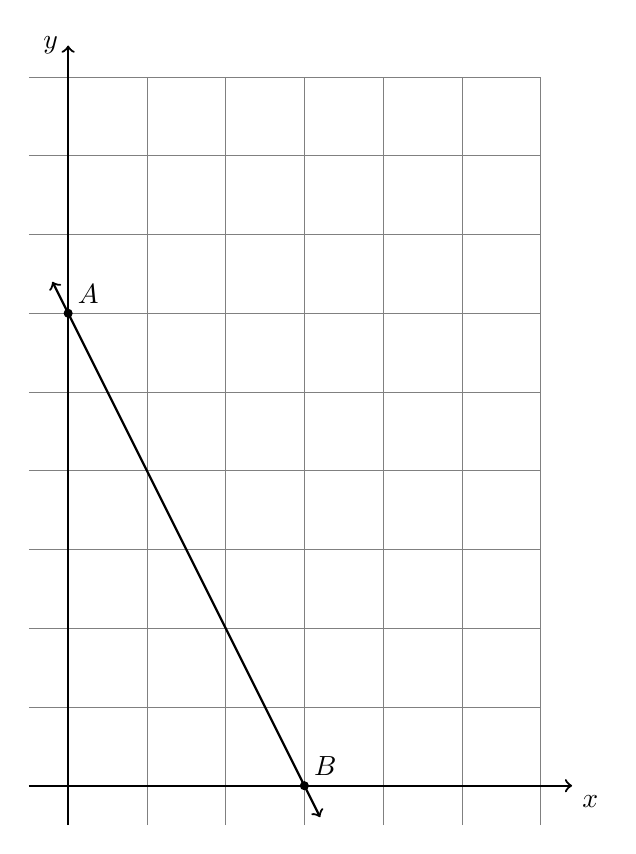
\begin{tikzpicture}
            \draw [help lines] (-0.5,-0.5) grid (6,9);
            \draw [thick, ->] (-0.5,0) -- (6.4,0) node [below right] {$x$};
            \draw [thick, ->] (0,-0.5)--(0,9.4) node [left] {$y$};
            \draw [thick, <->] (-0.2,6.4)--(3.2,-0.4);
            \draw [fill] (0,6) circle [radius=0.05] node[above right] {$A$};
            \draw [fill] (3,0) circle [radius=0.05] node[above right] {$B$};
          \end{tikzpicture}
        \end{center}
      \end{multicols}
    \end{enumerate} \vspace{2cm}

\item A triangle is dilated with factor $k$ such that $\triangle ABC \sim \triangle DEF$. Circle True or False.
    \begin{enumerate}[itemsep=0.5cm]
      \item T \quad F \quad $\angle A \cong \angle E$
      \item T \quad F \quad $\overline{AC} \rightarrow \overline{DF}$
      \item T \quad F \quad $\displaystyle k=\frac{DF}{AC}$
      \item T \quad F \quad $\overline{AC} \cong \overline{DF}$
      \item T \quad F \quad $\displaystyle \frac{DE}{AB} = \frac{EF}{BC}$
      \item T \quad F \quad $DE \times BC = AB \times EF$
    \end{enumerate}

\newpage
  \subsubsection*{Spicy: Using the distance formula to prove an isosceles triangle}
\item In this problem use the following theorem (copy it at the bottom of the page after your calculations): \\*[0.25cm]
    \emph{A triangle is isosceles if and only two of its sides are congruent.}\\*[0.5cm]
    Shown below is triangle $ABC$, $A(-2,2)$, $B(4,5)$, and $C(1,-1)$. \\*[0.25cm]
    Prove it is an isosceles triangle by
    \begin{enumerate}
      \item finding the length of each of the three sides,
      \item stating which sides are congruent,
      \item copying the theorem as your conclusion, adding \emph{therefore $\triangle ABC$ is isosceles}.
    \end{enumerate}
    \begin{flushright} %4 quadrant regents grid
      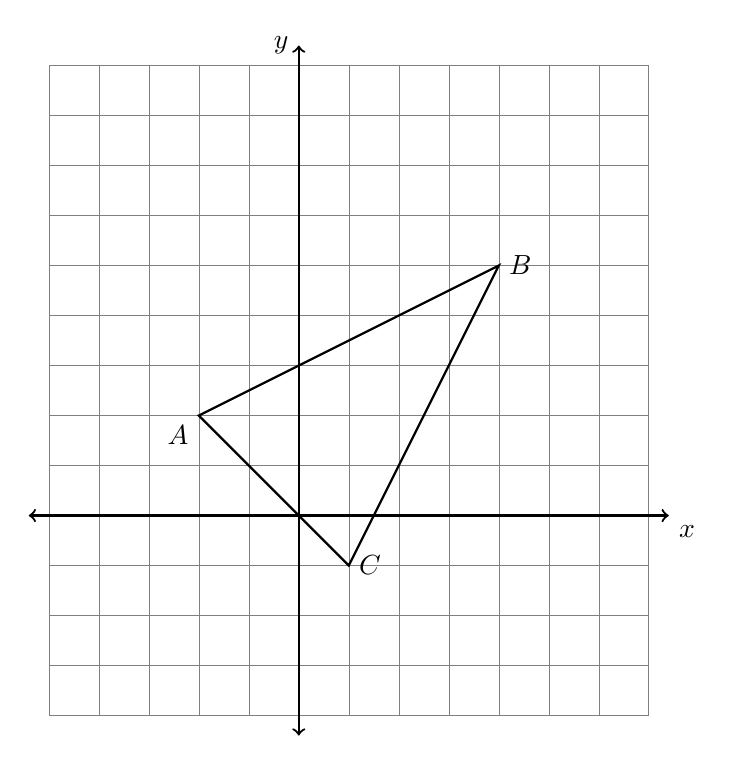
\begin{tikzpicture}[scale=.635]
        \draw [help lines] (-5,-4) grid (7,9);
        \draw [thick, <->] (-5.4,0) -- (7.4,0) node [below right] {$x$};
        \draw [thick, <->] (0,-4.4)--(0,9.4) node [left] {$y$};
        \draw [thick] (-2,2) node[below left] {$A$}--
        (4,5) node[right] {$B$}--
        (1,-1) node[right] {$C$}--cycle;
      \end{tikzpicture}
    \end{flushright}


\end{enumerate}
\end{document}